\section{Configureren}

Voor het opzetten van het project wordt er gebruik gemaakt van IntelliJ IDEA. Dit is een van de meest geadvanceerde \gls{IDE} die beschikbaar is op de markt. Deze \acrshort{IDE} maakt het moeiteloos om projecten die gebruik maken van onder andere Java en Kotlin op te zetten en te configureren. Bij het opzetten van een nieuw project is er de keuze om gebruik te maken van Maven of Gradle. Dit zijn allebei software project management tools die het mogelijk maken om externe libraries toe te voegen aan de codebase. In overleg met de andere afstudeerder hebben we ervoor gekozen om gebruik te maken van Maven, omdat we hier beide mee bekend zijn.

\subsection{Maven}

\begin{wrapfigure}[11]{r}{0.6\textwidth}
    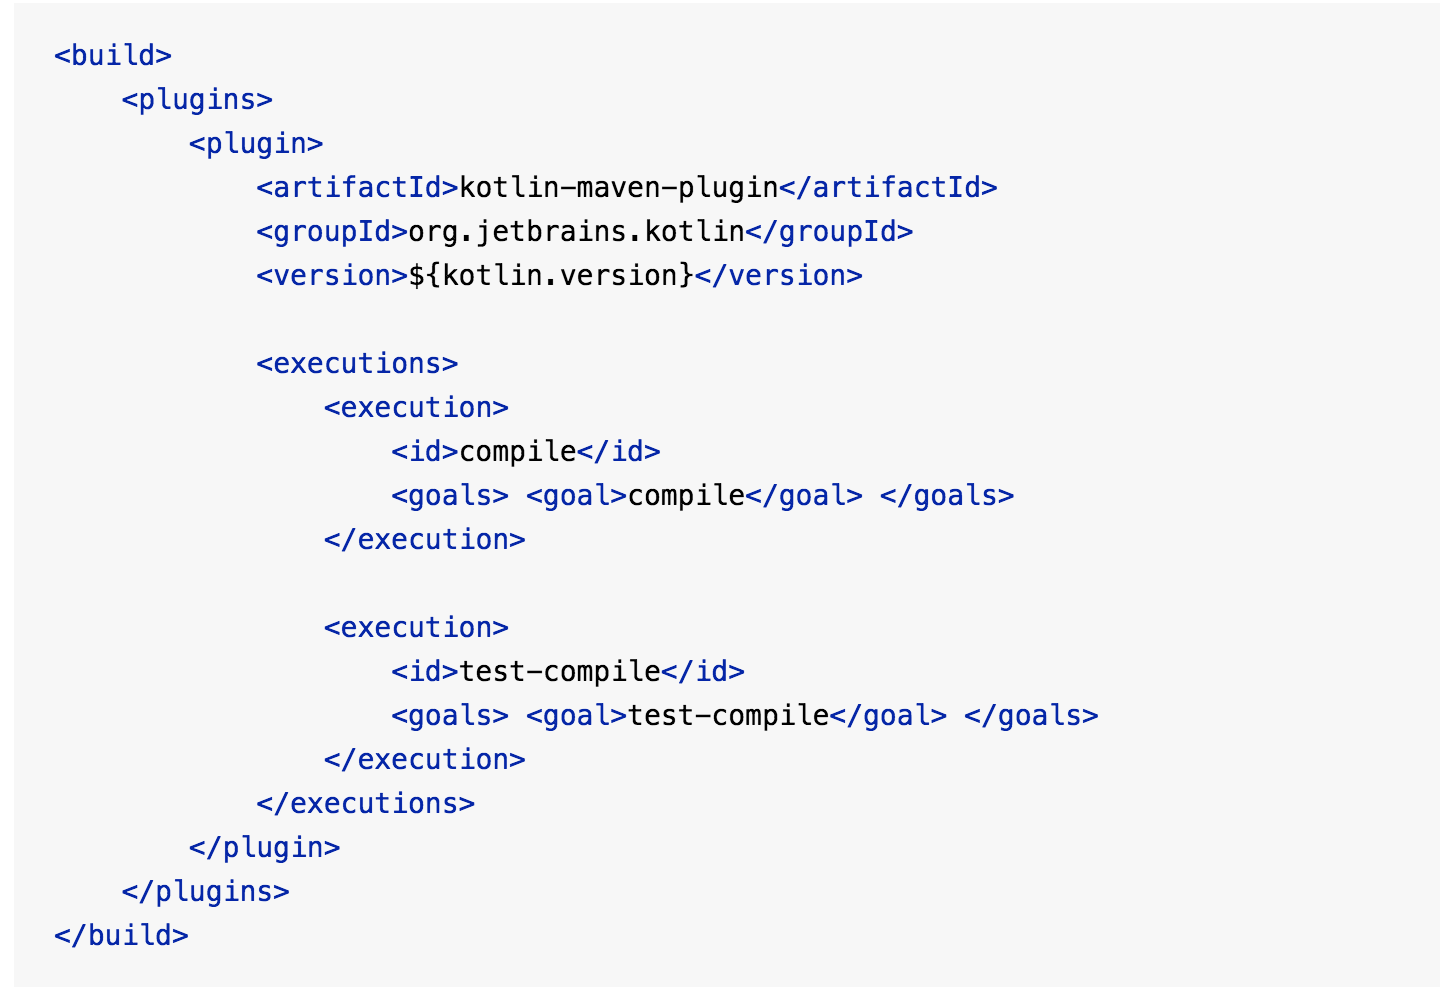
\includegraphics[width=0.6\textwidth, keepaspectratio]{figures/config-kotlin}
    \caption[Configuratie Maven]{Configuratie Maven in een Kotlin project afkomstig van ``Using Maven'' - \cite{kotlin_maven}.}
    \label{configuration:maven}
\end{wrapfigure} 

Tijdens de configuratie van Maven blijkt dat dit proces anders is als bij een Java project, waarbij je eigenlijk alleen een selectie hoeft te maken in de \acrshort{IDE}. Gelukkig is de documentatie van het Kotlin project op orde en is er snel gevonden wat er aangepast moet worden. In fig. \ref{configuration:maven} is te zien welk stuk toegevoegd moet worden in het configuratiebestand. Na dit gedaan te hebben worden libraries correct geïmporteerd.

\subsection{Docker}
oor het opzetten van een Docker image is er voor nu gekozen voor een simpele aanpak, waarbij we besloten hebben dat naarmate het project vordert, en wanneer nodig, het uitgebreid zal worden.

\begin{wrapfigure}[8]{l}{0.6\textwidth}
    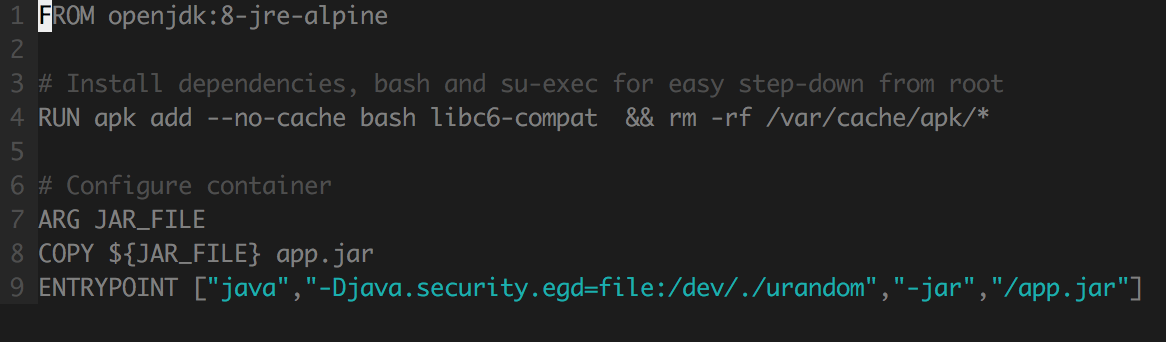
\includegraphics[width=0.6\textwidth, keepaspectratio]{figures/dockerfile}
    \caption[Configuratie Docker]{Opgestelde configuratie voor de Dockerfile.}
    \label{configuration:docker}
\end{wrapfigure} 

In fig. \ref{configuration:docker} is te zien hoe de Docker configuratie is opgezet. Er word gebruik gemaakt van een AlpineLinux gebaseerde image waarin de \acrfull{JDK} en de \acrfull{JRE} voorgeconfigureerd zijn. Voorlopig kopieërt het alleen maar de build artifact van het project naar de Docker omgeving, om het vervolgens op te starten.
